This appendix presents the comprehensive benchmark evaluation statistics across all 16 evaluated architectural pipeline configurations on the original, unconstrained raw enterprise knowledge corpus ($N = 100$). Unlike the closed corpus evaluated in Chapter~\ref{sec:results}, which was restricted to 1,701 pre-filtered chunks to match MuSiQue's candidate density, the raw corpus preserves the full uncurated scraped documentation (2,420 chunks with elevated real-world background noise).

\subsection{Execution Latency Profiles}
\label{subsec:raw_latency}
Table~\ref{tab:latency_enterprise_raw} reports the empirical Time to First Token (TTFT) and total execution latency distributions ($P_{50}$ and $P_{95}$) across all 16 pipeline architectures on the unconstrained corpus. To complement the tabular percentiles, Figure~\ref{fig:latency_breakdown_enterprise_raw} visualizes the corresponding component-wise mean latency breakdowns, isolating the execution duration consumed by vector retrieval, cross-encoder re-ranking ($M_2$), cache lookup overhead ($M_3$), query routing ($M_4$), and downstream token streaming.

\begin{table}[htbp]
\centering
\footnotesize
\renewcommand{\arraystretch}{0.93}
\setlength{\tabcolsep}{3.5pt}
\caption[Execution latency and TTFT profiles on raw Enterprise corpus]{End-to-end execution latency and Time-to-First-Token (TTFT) across 16 pipeline architectures on the unconstrained raw Enterprise corpus ($N = 100$). Statistical significance flags denote Holm-Bonferroni-adjusted paired Wilcoxon signed-rank tests against the naive baseline.}
\label{tab:latency_enterprise_raw}
\begin{tabular*}{\linewidth}{@{\extracolsep{\fill}} l r r r r r @{}}
\toprule
\textbf{Pipeline} & \makecell{\textbf{TTFT $P_{50}$}\\\scriptsize{(ms)}} & \makecell{\textbf{TTFT $P_{95}$}\\\scriptsize{(ms)}} & \makecell{\textbf{$T_{\text{total}} P_{50}$}\\\scriptsize{(ms)}} & \makecell{\textbf{$T_{\text{total}} P_{95}$}\\\scriptsize{(ms)}} & \makecell{\textbf{$\Delta T_{\text{total}}$}\\\scriptsize{(\%)}} \\
\midrule
\multicolumn{6}{@{}l@{}}{\textbf{Baseline ($k=0$)}} \\
Naive RAG Baseline & 1438.0 & 1780.0 & 1660.5 & 2320.2 & -- \\
\midrule
\multicolumn{6}{@{}l@{}}{\textbf{Single-Factor Isolated ($k=1$)}} \\
S2B & 1421.0 & 1779.6 & 1621.0 & 2257.3 & -2.4\%\textsuperscript{ns} \\
SR & 1616.0 & 2033.0 & 1802.5 & 2646.2 & +8.6\%\textsuperscript{***} \\
PC & 1694.5 & 2753.0 & 1969.0 & 3886.6 & +18.6\%\textsuperscript{***} \\
MC & 2008.5 & 11846.9 & 2208.5 & 11846.9 & +33.0\%\textsuperscript{***} \\
\midrule
\multicolumn{6}{@{}l@{}}{\textbf{Pairwise Combinations ($k=2$)}} \\
S2B + SR & 1764.5 & 3456.9 & 2020.0 & 3554.6 & +21.7\%\textsuperscript{***} \\
S2B + PC & 1520.0 & 2028.0 & 1682.5 & 2550.9 & +1.3\%\textsuperscript{ns} \\
S2B + MC & 1850.5 & 3337.0 & 2112.0 & 4016.8 & +27.2\%\textsuperscript{***} \\
SR + PC & 1615.0 & 2020.8 & 1762.0 & 2648.4 & +6.1\%\textsuperscript{***} \\
SR + MC & 2125.5 & 4495.5 & 2339.5 & 5007.1 & +40.9\%\textsuperscript{***} \\
PC + MC & 1940.5 & 3357.5 & 2159.5 & 3758.8 & +30.1\%\textsuperscript{***} \\
\midrule
\multicolumn{6}{@{}l@{}}{\textbf{Higher-Order Combinations ($k \ge 3$)}} \\
S2B + SR + PC & 1911.5 & 2875.8 & 2155.5 & 3093.9 & +29.8\%\textsuperscript{***} \\
S2B + SR + MC & 2246.0 & 4599.8 & 2444.5 & 4992.2 & +47.2\%\textsuperscript{***} \\
S2B + PC + MC & 2061.5 & 4046.6 & 2301.0 & 4447.7 & +38.6\%\textsuperscript{***} \\
SR + PC + MC & 2267.5 & 3967.1 & 2517.5 & 4523.6 & +51.6\%\textsuperscript{***} \\
S2B + SR + PC + MC & 2254.0 & 4083.2 & 2510.0 & 4730.5 & +51.2\%\textsuperscript{***} \\
\bottomrule
\end{tabular*}
\vspace{0.25em}
\parbox{\linewidth}{\scriptsize
\textbf{Notes:} $P_{50}$ and $P_{95}$ denote median and 95th percentile execution latencies. $\Delta T_{\text{total}}$ denotes percentage change relative to baseline. $^{*} p < 0.05, ^{**} p < 0.01, ^{***} p < 0.001$, $^{\mathrm{ns}} p \ge 0.05$ (paired Wilcoxon with Holm-Bonferroni correction vs. naive baseline).}
\end{table}


\begin{figure}[!htbp]
\centering
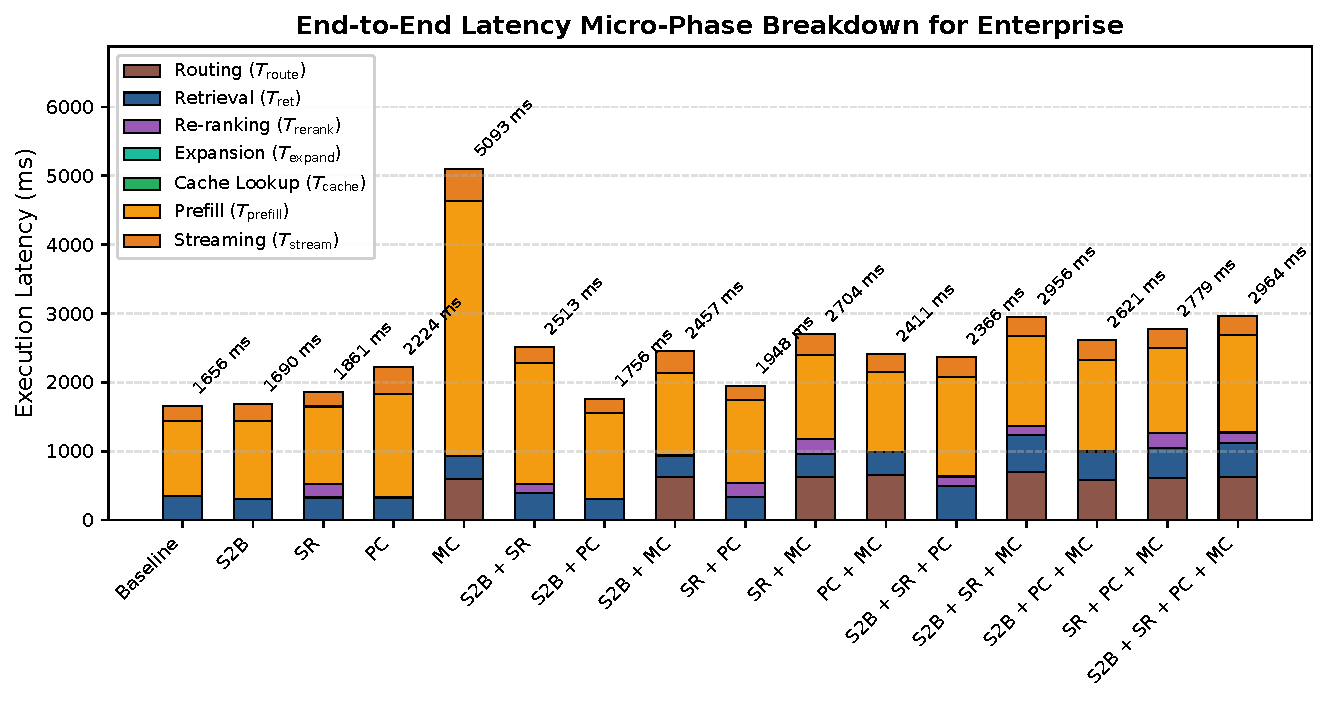
\includegraphics[width=0.94\linewidth]{figures/enterprise/latency_breakdown_enterprise.pdf}
\caption[Component-wise latency breakdown on raw Enterprise corpus]{Component-wise latency breakdown across all 16 pipeline configurations on the unconstrained raw enterprise corpus, detailing execution duration across retrieval, semantic re-ranking, cache management, and model tier generation phases. Stacked bars represent sample mean execution durations across queries, complementary to the median ($P_{50}$) profiles reported in Table~\ref{tab:latency_enterprise_raw}.}
\label{fig:latency_breakdown_enterprise_raw}
\end{figure}

\FloatBarrier
\subsection{Operational Expenditure Decompositions}
\label{subsec:raw_cost}
Table~\ref{tab:cost_enterprise_raw} summarizes the monetary operational expenditures incurred per 1,000 queries, detailing input token consumption, cache hit efficiency, and routing tier allocations under enterprise GCP pricing. The component-wise expenditure breakdown across uncached prompt prefill, context cache lookups, generative completion, and auxiliary neural re-ranking services is illustrated in Figure~\ref{fig:cost_breakdown_enterprise_raw}.

\begin{table}[htbp]
\centering
\footnotesize
\renewcommand{\arraystretch}{0.93}
\setlength{\tabcolsep}{3.5pt}
\caption{Operational cost and token consumption breakdown across 16 pipeline architectures on Enterprise. Statistical significance flags denote Holm-Bonferroni-adjusted paired Wilcoxon signed-rank tests against the naive baseline.}
\label{tab:cost_enterprise_raw}
\begin{tabular*}{\linewidth}{@{\extracolsep{\fill}} l r r r r r @{}}
\toprule
\textbf{Pipeline} & \makecell{\textbf{Uncached}\\\textbf{Prompt Tok}} & \makecell{\textbf{Cached}\\\textbf{Prompt Tok}} & \makecell{\textbf{Output}\\\textbf{Tokens}} & \makecell{\textbf{Cost / 1k}\\\scriptsize{(\$)}} & \makecell{\textbf{$\Delta$ Cost}\\\scriptsize{(\%)}} \\
\midrule
\multicolumn{6}{@{}l@{}}{\textbf{Baseline ($k=0$)}} \\
Naive RAG Baseline & 6,458 & 0 & 218 & \$5.662 & -- \\
\midrule
\multicolumn{6}{@{}l@{}}{\textbf{Single-Factor Isolated ($k=1$)}} \\
S2B & 7,525 & 0 & 190 & \$6.355 & +12.2\%\textsuperscript{ns} \\
SR & 5,852 & 0 & 168 & \$10.020 & +77.0\%\textsuperscript{*} \\
PC & 33 & 0 & 584 & \$6.817 & +20.4\%\textsuperscript{*} \\
MC & 6,458 & 0 & 163 & \$5.321 & -6.0\%\textsuperscript{ns} \\
\midrule
\multicolumn{6}{@{}l@{}}{\textbf{Pairwise Combinations ($k=2$)}} \\
S2B + SR & 7,895 & 0 & 226 & \$11.771 & +107.9\%\textsuperscript{*} \\
S2B + PC & 28 & 0 & 428 & \$7.027 & +24.1\%\textsuperscript{ns} \\
S2B + MC & 7,525 & 0 & 173 & \$6.338 & +11.9\%\textsuperscript{ns} \\
SR + PC & 26 & 0 & 380 & \$11.073 & +95.6\%\textsuperscript{*} \\
SR + MC & 5,849 & 0 & 141 & \$9.827 & +73.6\%\textsuperscript{*} \\
PC + MC & 24 & 0 & 323 & \$6.035 & +6.6\%\textsuperscript{ns} \\
\midrule
\multicolumn{6}{@{}l@{}}{\textbf{Higher-Order Combinations ($k \ge 3$)}} \\
S2B + SR + PC & 23 & 0 & 396 & \$12.181 & +115.1\%\textsuperscript{*} \\
S2B + SR + MC & 7,895 & 0 & 160 & \$11.277 & +99.2\%\textsuperscript{*} \\
S2B + PC + MC & 28 & 0 & 463 & \$6.988 & +23.4\%\textsuperscript{ns} \\
SR + PC + MC & 26 & 0 & 477 & \$10.472 & +84.9\%\textsuperscript{*} \\
S2B + SR + PC + MC & 23 & 0 & 440 & \$10.150 & +79.3\%\textsuperscript{ns} \\
\bottomrule
\end{tabular*}
\vspace{0.25em}
\parbox{\linewidth}{\scriptsize
\textbf{Notes:} Per-query sample token averages. Cost normalized per 1,000 queries based on Google Cloud Gemini enterprise tariffs. $\Delta\text{Cost}$ denotes percentage change relative to baseline. $^{*} p < 0.05, ^{**} p < 0.01, ^{***} p < 0.001$, $^{\mathrm{ns}} p \ge 0.05$ (paired Wilcoxon with Holm-Bonferroni correction vs. naive baseline).}
\end{table}


\begin{figure}[!htbp]
\centering
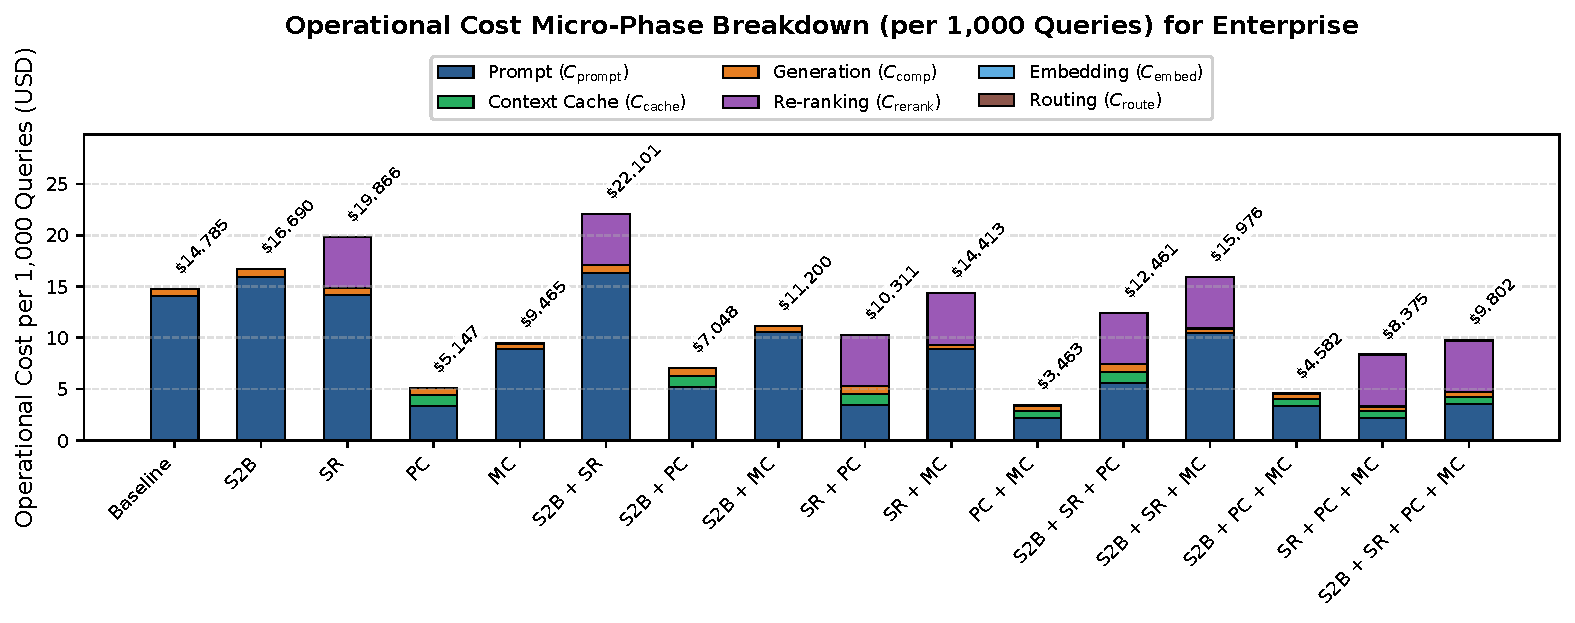
\includegraphics[width=0.94\linewidth]{figures/enterprise/cost_breakdown_enterprise.pdf}
\caption[Component-wise operational expenditure breakdown on raw Enterprise corpus]{Component-wise operational expenditure breakdown per 1,000 queries across all 16 pipeline configurations on the unconstrained raw enterprise corpus, detailing monetary expenditure across uncached context prefill, context cache lookups, generative completion, and auxiliary neural re-ranking services.}
\label{fig:cost_breakdown_enterprise_raw}
\end{figure}

\FloatBarrier
\subsection{Response Quality Profiles}
\label{subsec:raw_quality}
Table~\ref{tab:quality_enterprise_raw} details multi-dimensional retrieval and generation quality metrics (Context Precision, Context Recall, Faithfulness, Answer Relevancy, and Composite Quality $Q$) alongside false refusal rates. In this unconstrained environment with elevated distractor density, semantic re-ranking operates as an essential noise gate: combining Small-to-Big retrieval with re-ranking (S2B + SR and S2B + SR + PC) yields statistically significant quality improvements exceeding $+28\%$ over the naive baseline. Figure~\ref{fig:quality_lollipop_enterprise_raw} presents the corresponding configuration-level quality profiles across architectural tiers.

\begin{table}[htbp]
\centering
\scriptsize
\setlength{\tabcolsep}{2.2pt}
\caption{Retrieval, generation, and out-of-domain rejection quality metrics across 16 pipeline configurations on the Enterprise Knowledge Corpus ($N = 100$). Statistical significance flags denote Holm-Bonferroni-adjusted paired Wilcoxon signed-rank tests against the naive baseline ($C_0$).}
\label{tab:quality_enterprise}
\begin{tabular*}{\linewidth}{@{\extracolsep{\fill}} l l c c c c c c @{}}
\toprule
\textbf{Config} & \textbf{Pipeline} & \makecell{\textbf{Context}\\\textbf{Precision}} & \makecell{\textbf{Context}\\\textbf{Recall}} & \makecell{\textbf{Faithful-}\\\textbf{ness}} & \makecell{\textbf{Answer}\\\textbf{Relevancy}} & \makecell{\textbf{Rejection Acc. /}\\\textbf{Refusal $F_1$ (\%)}} & \makecell{\textbf{Composite}\\\textbf{Quality $Q$}} \\
\midrule
\multicolumn{8}{l}{\textbf{Baseline ($k=0$)}} \\
$C_{0}$ & Naive RAG Baseline & 0.693 & 0.917 & 0.750 & 0.631 & 100.0\% / 100.0\% & 0.6831 \\
\midrule
\multicolumn{8}{l}{\textbf{Single-Factor Isolated ($k=1$)}} \\
$C_{1}$ & S2B & 0.745 & 1.000 & 0.794 & 0.650 & 100.0\% / 100.0\% & \textbf{0.7355}\textsuperscript{ns} \\
$C_{2}$ & SR & 0.659 & 0.917 & 0.800 & 0.632 & 100.0\% / 100.0\% & 0.6599\textsuperscript{ns} \\
$C_{3}$ & PC & 0.641 & 0.917 & 0.149 & 0.820 & \phantom{00}0.0\% / \phantom{00}1.1\% & 0.2251\textsuperscript{ns} \\
$C_{4}$ & MC & 0.682 & 0.917 & 0.694 & 0.536 & 100.0\% / 100.0\% & 0.6001\textsuperscript{ns} \\
\midrule
\multicolumn{8}{l}{\textbf{Pairwise Combinations ($k=2$)}} \\
$C_{5}$ & S2B + SR & 0.783 & 0.933 & 0.790 & 0.653 & 100.0\% / 100.0\% & 0.7311\textsuperscript{ns} \\
$C_{6}$ & S2B + PC & 0.750 & 1.000 & 0.141 & 0.824 & \phantom{00}0.0\% / \phantom{00}1.0\% & 0.2649\textsuperscript{ns} \\
$C_{7}$ & S2B + MC & 0.750 & 1.000 & 0.788 & 0.638 & 100.0\% / 100.0\% & 0.7315\textsuperscript{ns} \\
$C_{8}$ & SR + PC & 0.649 & 0.917 & 0.065 & 0.818 & \phantom{00}0.0\% / \phantom{00}1.2\% & 0.1404\textsuperscript{ns} \\
$C_{9}$ & SR + MC & 0.690 & 0.917 & 0.800 & 0.646 & 100.0\% / 100.0\% & 0.6943\textsuperscript{ns} \\
$C_{10}$ & PC + MC & 0.651 & 0.917 & 0.166 & 0.829 & \phantom{00}0.0\% / \phantom{00}1.1\% & 0.2456\textsuperscript{ns} \\
\midrule
\multicolumn{8}{l}{\textbf{Higher-Order Triplets \& Full-Stack ($k \ge 3$)}} \\
$C_{11}$ & S2B + SR + PC & 0.783 & 0.933 & 0.149 & 0.832 & \phantom{00}0.0\% / \phantom{00}1.1\% & 0.3096\textsuperscript{ns} \\
$C_{12}$ & S2B + SR + MC & 0.758 & 0.933 & 0.788 & 0.637 & 100.0\% / 100.0\% & 0.7191\textsuperscript{ns} \\
$C_{13}$ & S2B + PC + MC & 0.745 & 1.000 & 0.237 & 0.821 & \phantom{00}0.0\% / \phantom{00}1.0\% & 0.3203\textsuperscript{ns} \\
$C_{14}$ & SR + PC + MC & 0.651 & 0.917 & 0.080 & 0.816 & \phantom{00}0.0\% / \phantom{00}1.2\% & 0.1545\textsuperscript{ns} \\
$C_{15}$ & S2B + SR + PC + MC (Full-Stack) & 0.843 & 0.926 & 0.327 & 0.817 & \phantom{00}0.0\% / \phantom{00}1.5\% & 0.4253\textsuperscript{ns} \\
\bottomrule
\end{tabular*}
\vspace{0.5em}
\parbox{\linewidth}{\footnotesize
\textbf{Notes:} Context Precision, Context Recall, Faithfulness, and Answer Relevancy are evaluated via RAGAS~\citep{es2024ragas}. Rejection Accuracy evaluates adherence in refusing unanswerable out-of-domain (OOD) queries, with Refusal $F_1$ assessing lexical precision against reference refusal templates. Composite Quality $Q \in [0, 1]$ represents the regularized harmonic mean across the four RAGAS dimensions (Equation~\ref{eq:composite_quality}, $\epsilon = 10^{-4}$). Statistical significance flags denote two-tailed paired Wilcoxon signed-rank tests against baseline ($C_0$) with Holm-Bonferroni correction ($^{*} p < 0.05$, $^{**} p < 0.01$, $^{***} p < 0.001$, $\mathrm{ns} = p \ge 0.05$).}
\end{table}


\begin{figure}[!htbp]
\centering
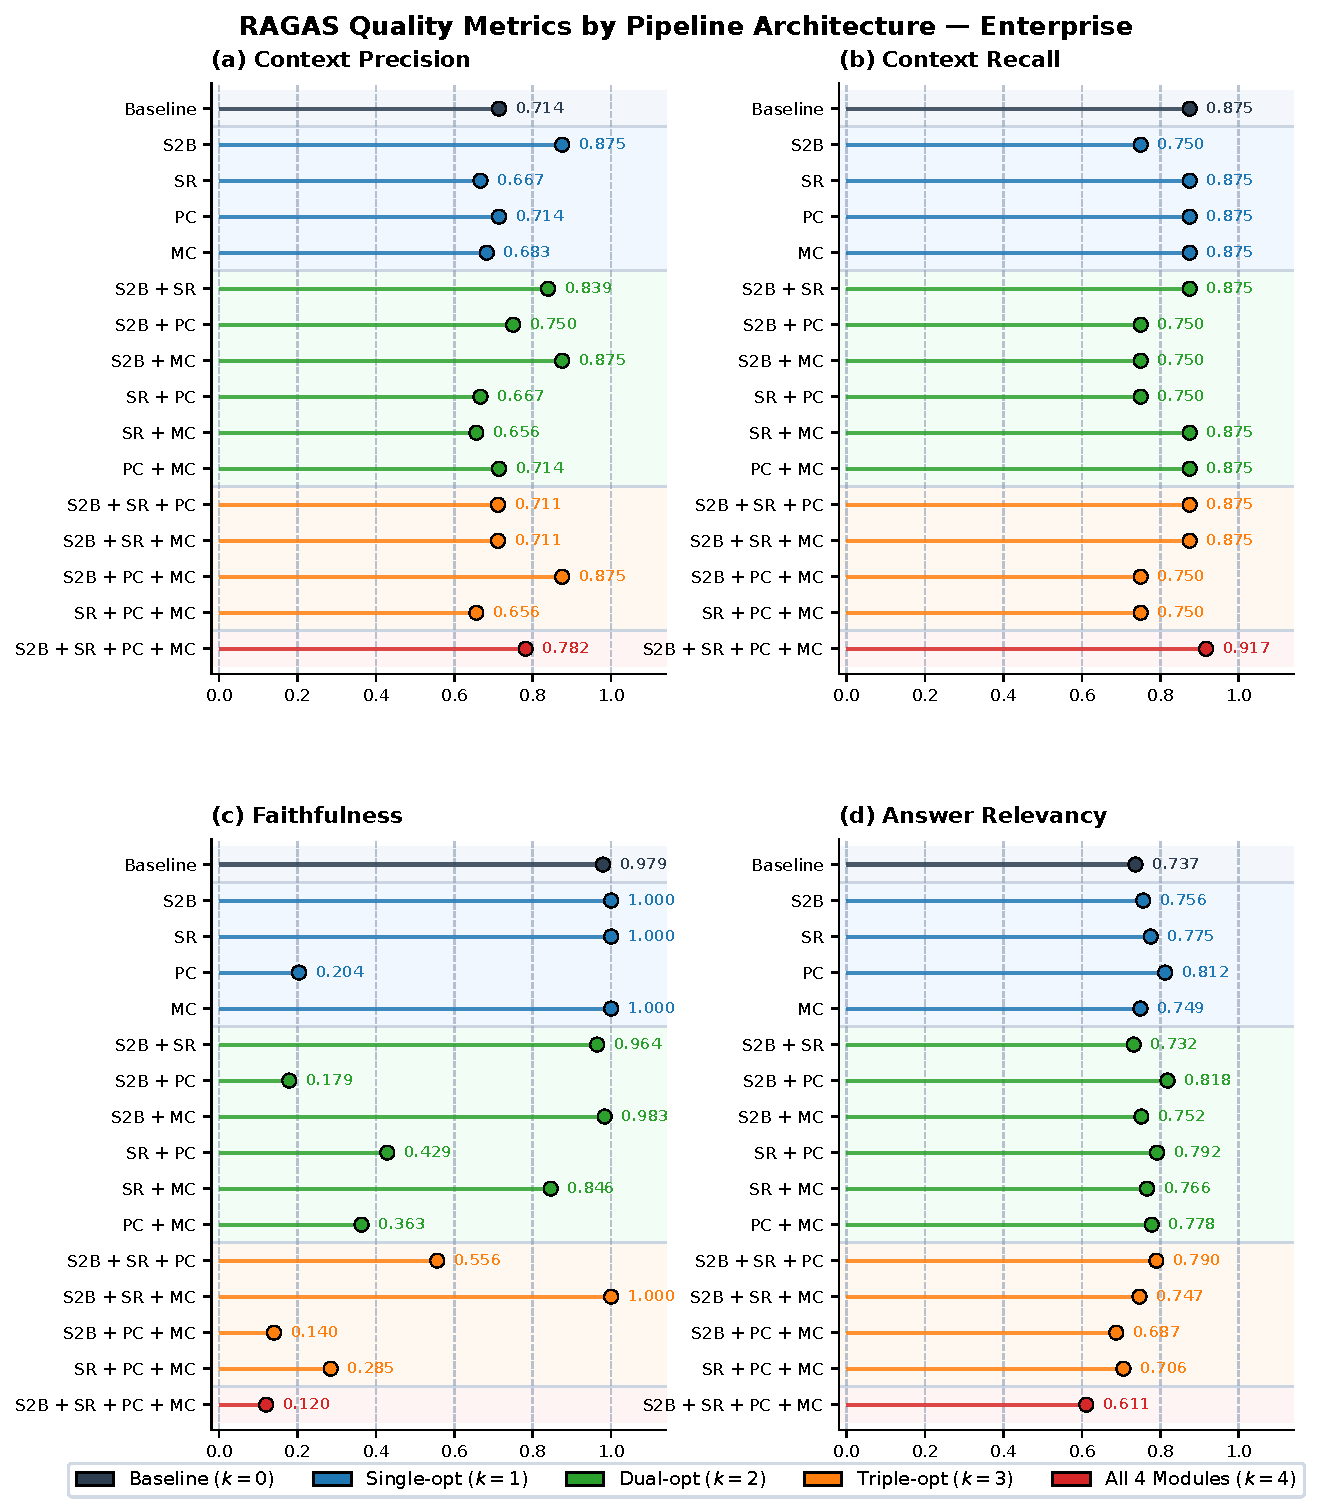
\includegraphics[width=0.85\linewidth]{figures/enterprise/quality_lollipop_enterprise.pdf}
\caption[Multi-dimensional response quality profiles on raw Enterprise corpus]{Multi-dimensional response quality profiles across architectural configurations on the unconstrained raw enterprise corpus, comparing Context Precision, Context Recall, Faithfulness, and Answer Relevancy across architectural tiers ($k=0 \dots 4$). Horizontal lollipop plots with tier-stratified background shading isolate configuration-level variations.}
\label{fig:quality_lollipop_enterprise_raw}
\end{figure}

\FloatBarrier
\subsection{Empirical Pareto Frontiers}
\label{subsec:raw_pareto}
Table~\ref{tab:pareto_enterprise_raw} and Figure~\ref{fig:pareto_frontier_enterprise_raw} illustrate the empirical 3D Pareto frontier balancing Composite Quality ($Q$), median execution latency ($T_{\text{total}}\ P_{50}$), and operational expenditure ($\text{Cost}_{1\text{k}}$) on the unconstrained raw enterprise corpus. Solid lines delineate the non-dominated Pareto frontier across configurations.

\begin{table}[htbp]
\centering
\footnotesize
\renewcommand{\arraystretch}{0.93}
\setlength{\tabcolsep}{3.5pt}
\caption[Multi-objective Pareto efficiency metrics on raw Enterprise corpus]{Multi-objective Pareto efficiency and 3D non-domination trade-off metrics across 16 pipeline architectures on the unconstrained raw Enterprise corpus ($N = 100$).}
\label{tab:pareto_enterprise_raw}
\begin{tabular*}{\linewidth}{@{\extracolsep{\fill}} l c r r r r c @{}}
\toprule
\textbf{Pipeline} & \makecell{\textbf{Composite}\\\textbf{Quality $Q$}} & \makecell{\textbf{Cost / 1k}\\\scriptsize{(\$)}} & \makecell{\textbf{$T_{\text{total}} P_{50}$}\\\scriptsize{(s)}} & \textbf{QPD} & \textbf{QPS} & \makecell{\textbf{Pareto}\\\textbf{Optimal}} \\
\midrule
\multicolumn{7}{@{}l@{}}{\textbf{Baseline ($k=0$)}} \\
Naive RAG Baseline & 0.5022 & \$14.785 & 1.66 & 34 & 0.30 & \textbf{Yes} \\
\midrule
\multicolumn{7}{@{}l@{}}{\textbf{Single-Factor Isolated ($k=1$)}} \\
S2B & 0.6368 & \$16.690 & 1.62 & 38 & 0.39 & \textbf{Yes} \\
SR & 0.5479 & \$19.866 & 1.80 & 28 & 0.30 & No \\
PC & 0.5326 & \$5.147 & 1.97 & 103 & 0.27 & \textbf{Yes} \\
MC & 0.5149 & \$9.465 & 2.21 & 54 & 0.23 & No \\
\midrule
\multicolumn{7}{@{}l@{}}{\textbf{Pairwise Combinations ($k=2$)}} \\
S2B + SR & 0.6433 & \$22.101 & 2.02 & 29 & 0.32 & No \\
S2B + PC & 0.6633 & \$7.048 & 1.68 & 94 & 0.39 & \textbf{Yes} \\
S2B + MC & 0.6492 & \$11.200 & 2.11 & 58 & 0.31 & No \\
SR + PC & 0.5688 & \$10.311 & 1.76 & 55 & 0.32 & No \\
SR + MC & 0.5596 & \$14.413 & 2.34 & 39 & 0.24 & No \\
PC + MC & 0.5634 & \$3.463 & 2.16 & 163 & 0.26 & \textbf{Yes} \\
\midrule
\multicolumn{7}{@{}l@{}}{\textbf{Higher-Order Combinations ($k \ge 3$)}} \\
S2B + SR + PC & 0.6466 & \$12.461 & 2.16 & 52 & 0.30 & No \\
S2B + SR + MC & 0.6162 & \$15.976 & 2.44 & 39 & 0.25 & No \\
S2B + PC + MC & 0.6268 & \$4.582 & 2.30 & 137 & 0.27 & \textbf{Yes} \\
SR + PC + MC & 0.5434 & \$8.375 & 2.52 & 65 & 0.22 & No \\
S2B + SR + PC + MC & 0.6028 & \$9.802 & 2.51 & 61 & 0.24 & No \\
\bottomrule
\end{tabular*}
\vspace{0.25em}
\parbox{\linewidth}{\scriptsize
\textbf{Notes:} Composite Quality $Q \in [0, 1]$ (Eq.~\ref{eq:composite_quality}). $\text{QPD} = Q / \text{Cost}_{1\text{k}}$ and $\text{QPS} = Q / T_{\text{total}}$ represent resource efficiency ratios. Pareto optimality denotes 3D non-domination ($\max Q, \min \text{Cost}, \min T_{\text{total}}$). Bold indicates Pareto-optimal configuration.}
\end{table}


\begin{figure}[!htbp]
\centering
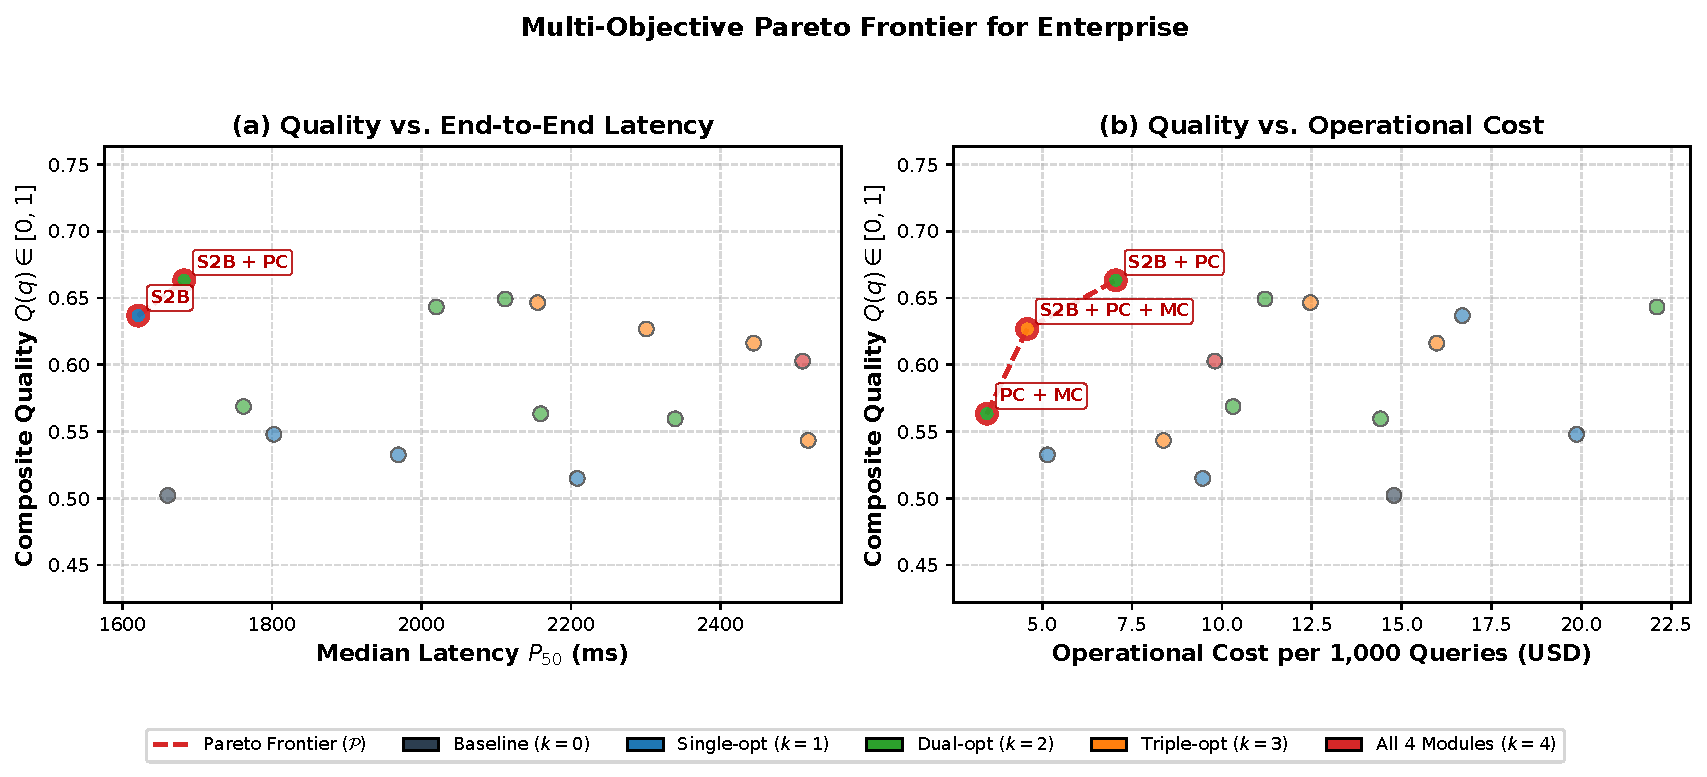
\includegraphics[width=0.90\linewidth]{figures/enterprise/pareto_frontier_enterprise.pdf}
\caption[Empirical Pareto frontier on raw Enterprise corpus]{Empirical Pareto frontier of Composite Quality ($Q$) versus median end-to-end execution latency ($T_{\text{total}}\ P_{50}$) and operational expenditure ($\text{Cost}_{1\text{k}}$) on the unconstrained raw enterprise corpus. Solid lines delineate the non-dominated empirical Pareto frontier across configurations.}
\label{fig:pareto_frontier_enterprise_raw}
\end{figure}
